Looking back through the thesis, What was researched, compared, investigated, designed, developed, and estimated are now exceeding the completion of a blockchain-based application. During the process of whole research, I have been constantly inspired to think various problems far beyond the project itself. So in this chapter, it was constructed by my insights, thoughts, and Outlook.

\section{When to Use Blockchain}
Like Maslow once said "if the only tool you have is a hammer,to treat everything as if it were a nail." In the software industry we repeatedly find new and cool hammers and then try to hit as many nails as we can. And the new one now is Blockchain. Today the media a little bit exaggerate the capability of Blockchain technologies, you can easily find out massive blockchain-embedded solution in many field. However blockchain isn't panacea, thus it is necessary to evaluate if blockchain technology is right for a particular project.

\subsection{Factors to Consider}
So before any enterprise makes up their mind of adopting Blockchain techlogies, it is necessary to conduct a comprehensive estimation whether applyin Blockchain or not. Hyperledger Technologies Organization gives generalized, high-level decision points about when to use or not to use blockchain technology (Figure 8.1)
\begin{figure}[htb]% order of placement preference: here, top, bottom
	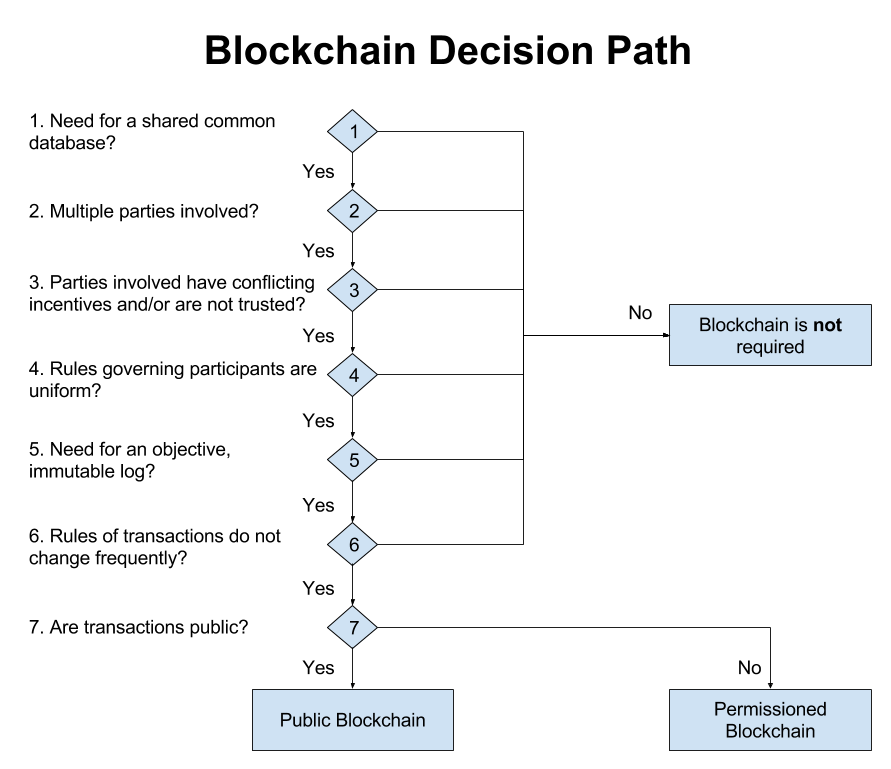
\includegraphics[width=\textwidth]{charts/Blockchain_Decision_Flowchart}
	\caption{Blockchain Decision Flowchart \cite{decision}}
\end{figure}
Comparing with when is suitable for using blockchain, when is \textbf{NOT} requires our caution more. Those are some conditions which are not suitable to develop blockchain-based soltions:
\begin{itemize}
	\item Business logic changes frequently\\
		- The smart contract is pre-set in the Nodes, frequent change may cause the failure of the system.
	\item Strict confidentiality\\
		- In the permissionless Blockchain platforms, the data is transparent to anyone. Even permissioned Blockchains with special mechanism to increase the privacy, like Corda and Hyperledger Ledger, the data is still at least known to the involved parties. Business with low tolerance for data transparency is not suitable for using blockchain. 
	\item Large Data Exchange \& Storage \\
		- In Blockchain system, the ledgers are fully or partly(like Corda) stored in each Nodes. The rate of repetition is rather highly, thus it is suitable for systems only storing the minimum necessary information, without too much data exchange in each transaction.\\
	\item Better alternatives\\
		- If there exists simpler, more mature options, it would be more effective.
\end{itemize}
 
\section{Summary}
The 6-month master thesis is until here almost to an end. It all stared with an occasion that 5 years ago I stumbled upon the term "Bitcoin", and later I got to have deeper insights about the blockchain technology. However, it took quite considerable time to find the satisfying research orientation. Yet it was only the tip of an iceberg, during research and development, there always sprang up unexpected challenges, and countless hours with effort were invested. In retrospect, considering the obstacles overcome, the result achieved, and the valuable reference information provided, all the work was worthwhile.

\subsection{What Were Accomplished}
The master thesis started from doing research about how far have the applications of blockchain technology proceeded in diverse fields, how practical they are. Among the wide range of fields, the application in supply chain has been chosen to be the object of study.
Logistics is a very important part of supply chain, it controls the delivery ability and circulation. To be specific, how to manage the Turnover Boxes efficiently, robustly, transparently and automatically is the core issue. Thus using blokchain as the tool to solve the pain point.\\

Before I started the project, I have been dived into the blockchain platform pool aiming to get the first-hand information for the application. In the end, the two candidates: Hyperledger Fabric and Corda haven been chosen to realized the Turnover Box System. The purpose was to find out the best suitable platform to build the Turnover Box System, and provide first-hand information for the companies having the similar business logic to help them build their own blockchain applications\\

After 3-4 months development, the CorDapp has successfully come into use, which works as well as expected before. The developing plan on Hyperledger Fabric has been pruned. In the previous chapters, the details of design, development, test and evaluation on this CorDapp have demonstrated Corda is the optimal choice for the Turnover Box System.\\

 
\subsection{Why Corda not Hyperledger Fabric}
Though in the previous chapter, the comparison between Hyperledger Fabric and Corda has been listed. Those differences are only from the theoretical analysis. After the involvement in both platform, there are some reasons why the Corda is more suitable than Hyperledger Fabric from the developers' perspective.
\begin{itemize}
	\item Higher Prerequisites \\
	- Hyperledger Fabric requires more dependencies, the smart contracts ("chaincode") run within a container environment(e.g Docker). Usually a single wrongly installed version of the tools will cause errors.
	\item Complex configuration \\
	- in order to set up the Hyperledger Fabric network, Hyperledger Fabric platform-specific binaries, docker images should be installed. The docker configuration file is rather tedious and no clear clue to guide.
	\item Unstable version update \\
	- Usually when a new version of the platform arrives, most of previous dependencies won't work at all and need to be updated. The docker images' frequent changed locations will also cause a lot of "Not Find" errors.  
	\item Bad Documentation \\
	- Frequent change but slow update in documentation, which usually results in the invalid links on the web page. No precise guidance in configuration and development.
\end{itemize}
Comparing with Hyperleger Fabric, the corda is relatively compact, flexible and efficient with reduced prerequisites, dependencies and usage of JVM.

\section{Outlook}
Today the blockchain on the one hand has been highly praised, on the other hand has been taken as hype suspect. After having had a close touch with it, I prefer to see the more positive side. The call for lower-cost management, traceability, transparency and automation will only increase. What's more, I would love to see more involvement of other flourish technologies. Like quantum computers help to improve the performance, 5G will broaden the bandwidth, and embracing IoT will realize the fully automation "machine talks to machine". The blockchain technology used in Turnover Box System can seamlessly extend to the whole supply chain, we expect to the fully connect network with highly automation and efficiency. 
Who expected that the simple "ALOHA" would raise the huge wave of Internet which vastly changes our World. \\


I am very excited to see what future brings. 


